\documentclass{beamer}

\mode<presentation> {
\usetheme{Singapore}
\setbeamercovered{transparent}

%\setbeamertemplate{footline} % To remove the footer line in all slides uncomment this line
%\setbeamertemplate{footline}[page number] % To replace the footer line in all slides with a simple slide count uncomment this line
%\setbeamertemplate{navigation symbols}{} % To remove the navigation symbols from the bottom of all slides uncomment this line
}

\usepackage{xeCJK}
\usepackage{fontawesome}
\usepackage{graphicx} 
\usepackage{booktabs} 
\usepackage{xcolor}
\usepackage{calc}
\usepackage{amsmath}
\usepackage{subfigure}

\setbeamertemplate{caption}[numbered]
\AtBeginEnvironment{figure}{\setcounter{subfigure}{0}}

% Chinese fonts.
\setCJKmainfont{FandolKai}

% \makeatletter
% \setbeamertemplate{frametitle}{
%     \ifbeamercolorempty[bg]{frametitle}{}{\nointerlineskip}%
%     \@tempdima=\textwidth%
%     \advance\@tempdima by\beamer@leftmargin%
%     \advance\@tempdima by\beamer@rightmargin%
%     \vspace*{1cm} %%%%%%%%%%%%% For example insert shift to right
%     \begin{beamercolorbox}[sep=0.3cm,center,wd=\the\@tempdima]{frametitle}
%         \usebeamerfont{frametitle}%
%         \vbox{}\vskip-1ex%
%         \if@tempswa\else\csname beamer@ftecenter\endcsname\fi%
%         {%
%             \ifx\insertframesubtitle\@empty%
%             \else%
%             {\usebeamerfont{framesubtitle}\usebeamercolor[fg]{framesubtitle}\insertframesubtitle\strut\par}%
%             \fi
%         }%
%         \vskip-1ex%
%         \if@tempswa\else\vskip-.3cm\fi% set inside beamercolorbox... evil here...
%     \end{beamercolorbox}%
% }
% \makeatother

\newcommand{\maincolorRGB}{39, 32, 99}
\definecolor{maincolor}{RGB}{\maincolorRGB}
\newcommand{\ctextbf}[1]{\textbf{\textcolor{maincolor}{\normalsize{#1}}}}

\newcommand{\vect}[1]{\boldsymbol{#1}}
\newcommand{\matr}[1]{\mathbf{#1}}
\newcommand{\lnn}[1]{
  \ln\left(#1\right)
}

\newlength\dlf
\newcommand\alignedbox[2]{
  % #1 = before alignment
  % #2 = after alignment
  &
  \begingroup
  \settowidth\dlf{$\displaystyle #1$}
  \addtolength\dlf{\fboxsep+\fboxrule}
  \hspace{-\dlf}
  \fcolorbox{red}{yellow}{$\displaystyle #1 #2$}
  \endgroup
}

\pgfdeclareimage[height=0.7cm]{company-logo}{img/realtek.png}
\logo{\pgfuseimage{company-logo}}

\author{\huge{許子駿}\\\LARGE{Oscar}} 
\institute[] 
{
    \scriptsize{
        \href{tel:+886-987605719}{ \raisebox{-0.1\height}\faPhone\ \underline{+886-987605719} ~} 
        \href{mailto:vm3y3rmp40719@gmail.com}{\raisebox{-0.2\height}\faEnvelope\  \underline{tzuchunhsu@realtek.com}} \\~\\
        \href{https://www.linkedin.com/in/tzu-chun-hsu-ab4b3b188/}{\raisebox{-0.2\height}\faLinkedinSquare\ \underline{tzu-chun-hsu-ab4b3b188} ~}
        \href{https://github.com/Oscarshu0719}{\raisebox{-0.2\height}\faGithub\ \underline{Oscarshu0719}}
    }
}
\date{Feb. 27, 2025} 

\begin{document}

\begin{frame}
\titlepage % Print the title page as the first slide
\end{frame}

% \begin{frame}
% \frametitle{Table of contents} 
% \tableofcontents 
% \end{frame}

%----------------------------------------------------------------------------------------
%	EDUCATION SLIDES
%----------------------------------------------------------------------------------------

\section{Education}
\begin{frame}
    \frametitle{Education}
    \begin{block}{Zhejiang University} % #47 QS 2025.
        Bachelor of Engineering in Computer Science and Technology\\
        Hangzhou, China \hfill 09 2016 – \ 07 2020
    \end{block}
    \begin{block}{National Yang Ming Chiao Tung University}
        Master of Science in Computer Science and Engineering\\
        Hsinchu, Taiwan \hfill 09 2022 – \ 02 2025
    \end{block}
\end{frame}

%----------------------------------------------------------------------------------------
%	PROJECTS SLIDES
%----------------------------------------------------------------------------------------

\section{Projects}
\begin{frame}
    \frametitle{Projects}
    \begin{block}{}
        \begin{enumerate}
            \item Chord learning and adversarial framework for symbolic music generation.
            \item Voice Conversion Based on Generative Adversarial Networks.
            \item Synthetic Data Generation using Conditional Normalizing Flows.
        \end{enumerate}

        \begin{figure}[H]
            \centering
            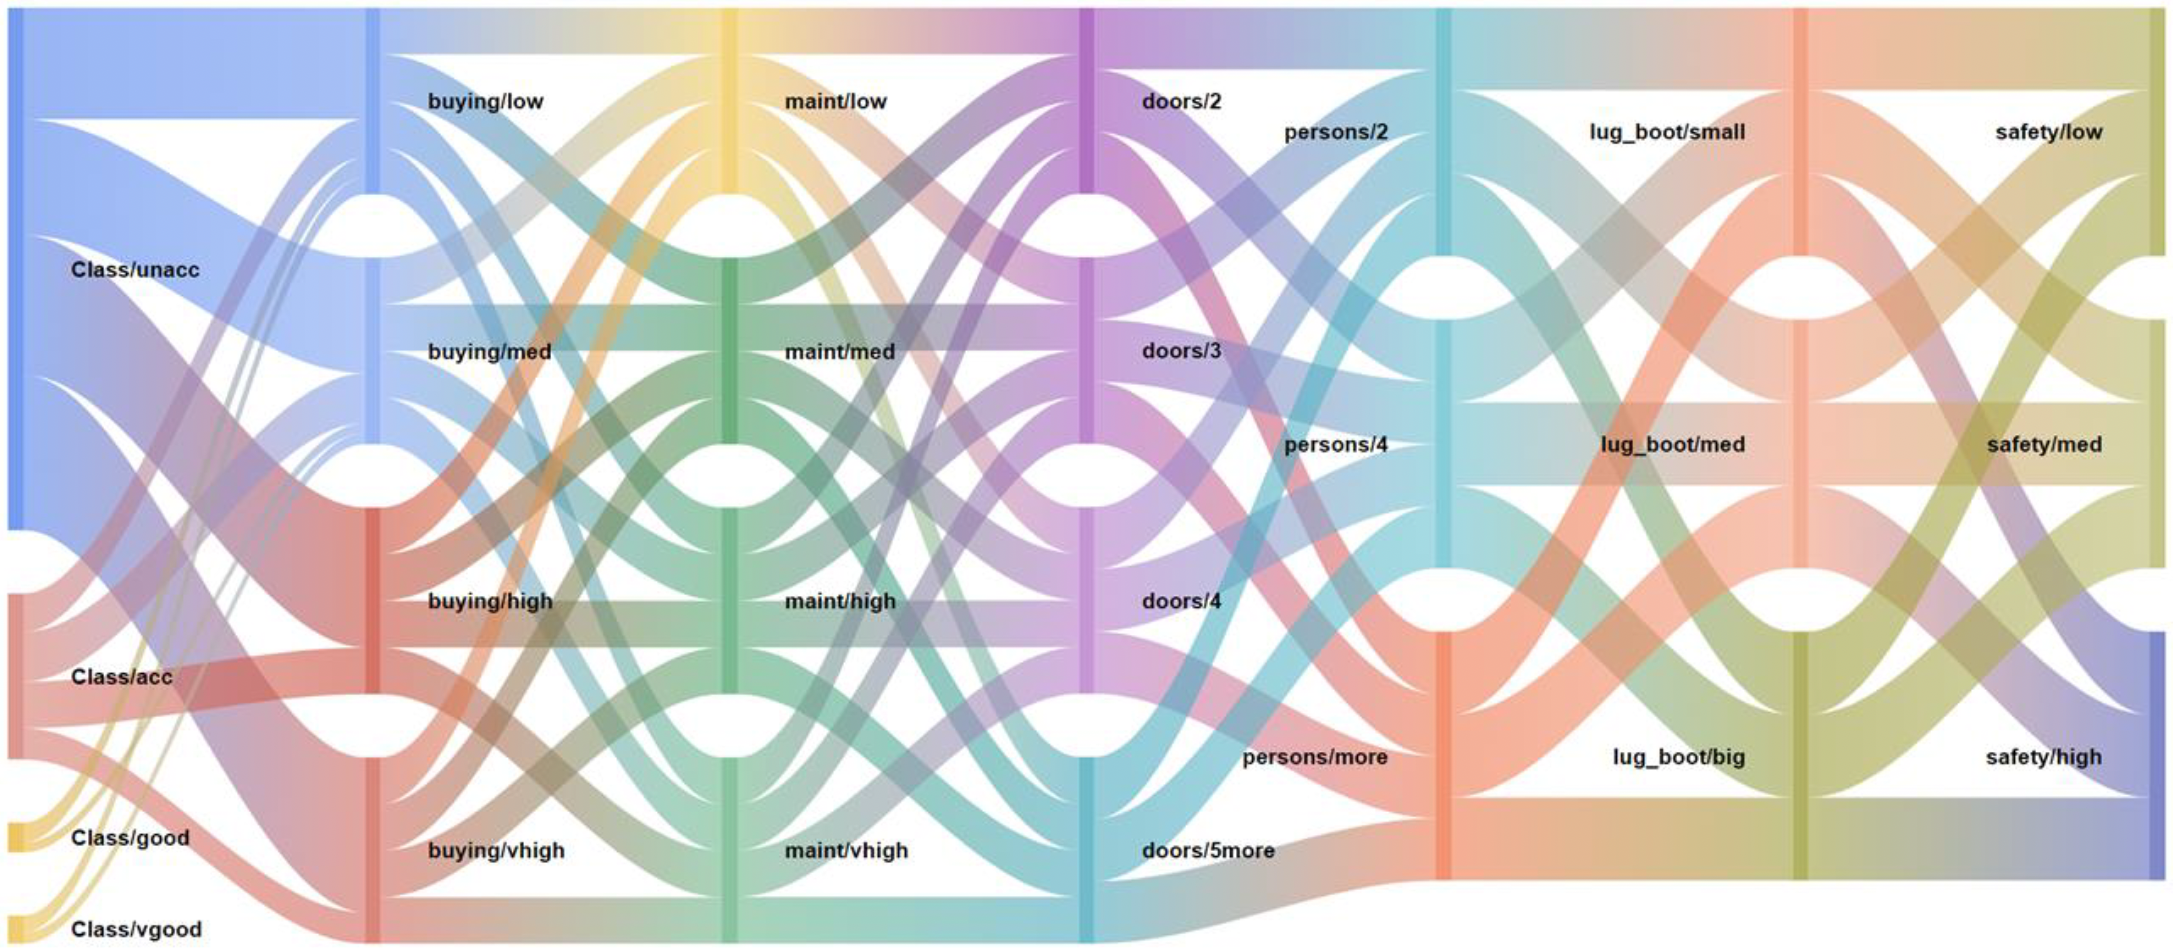
\includegraphics[scale=0.19]{img/cnf.png}
            \caption{Sankey diagram example}
        \end{figure}
    \end{block}
\end{frame}

\begin{frame}
    \frametitle{Projects}
    \begin{block}{4. Floating image quality compensation algorithm technology}
        \begin{figure}
            \only<1>{
                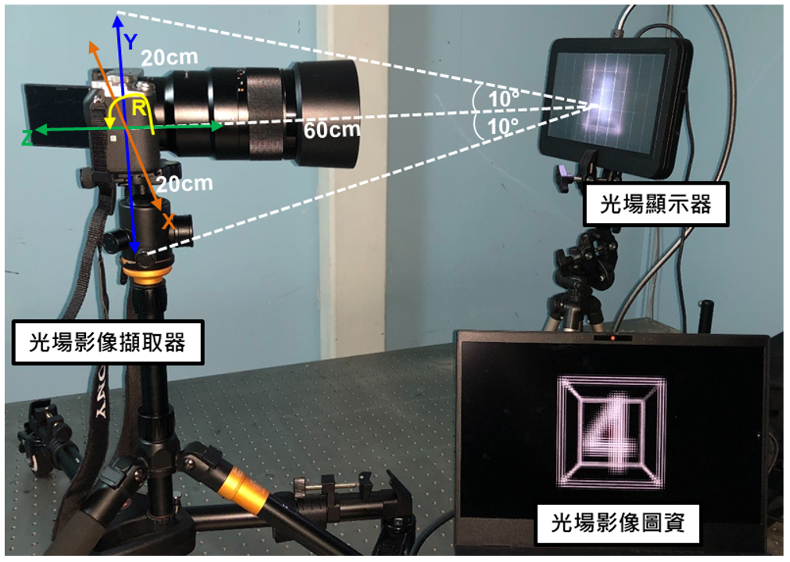
\includegraphics[scale=0.5]{img/device.png}
                \caption{Our floating image display system}
            }
            \setcounter{figure}{2}
            \only<2>{
                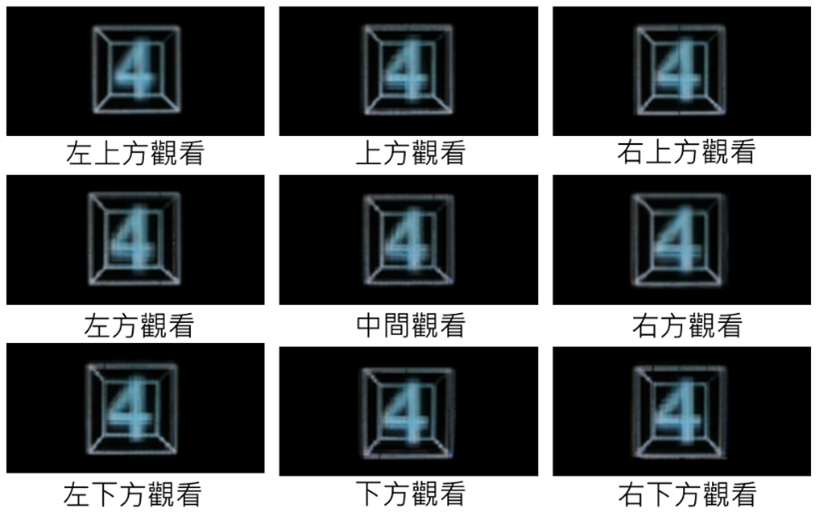
\includegraphics[scale=0.8]{img/imaging-views.png}
                \caption{9 different views sample}
            }
            \setcounter{figure}{3}
            \only<3>{
                \subfigure[Mismatch]{
                    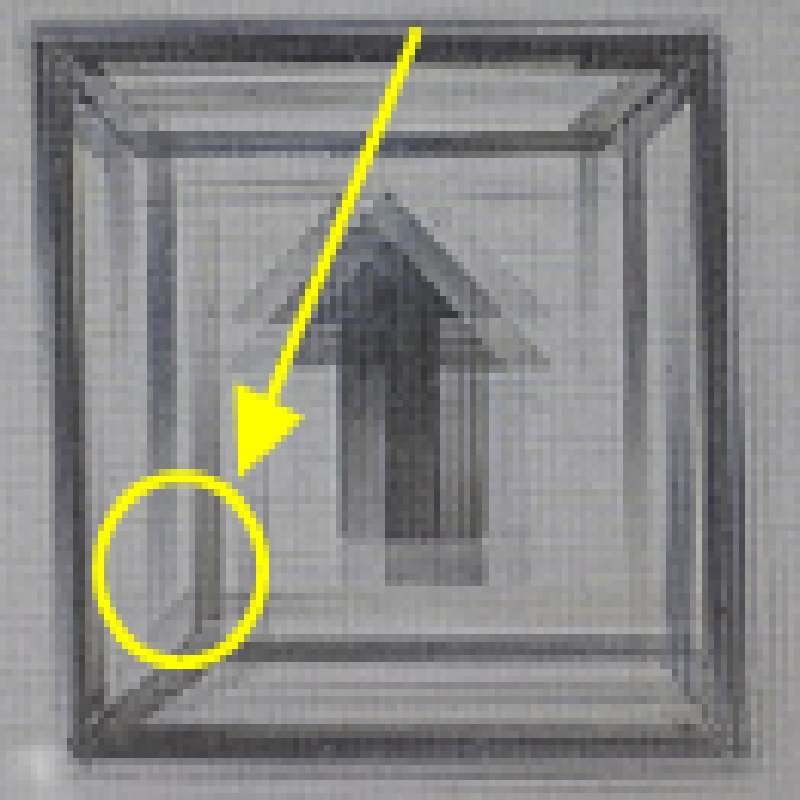
\includegraphics[width=0.3\textwidth]{img/imperfections-1.png}
                }
                \subfigure[Distortion]{
                    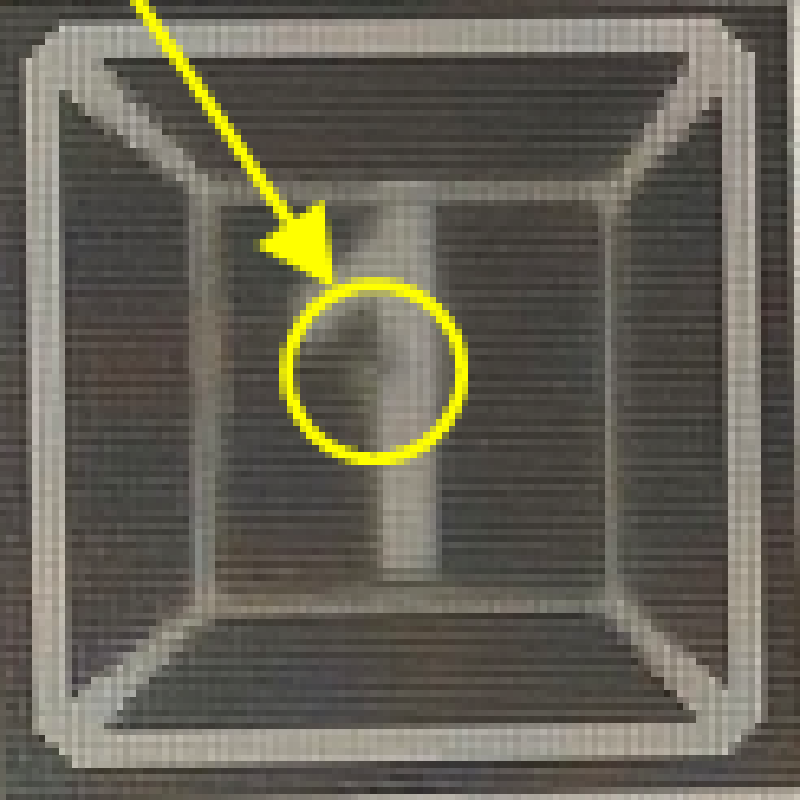
\includegraphics[width=0.3\textwidth]{img/imperfections-2.png}
                }
                \subfigure[Blur]{
                    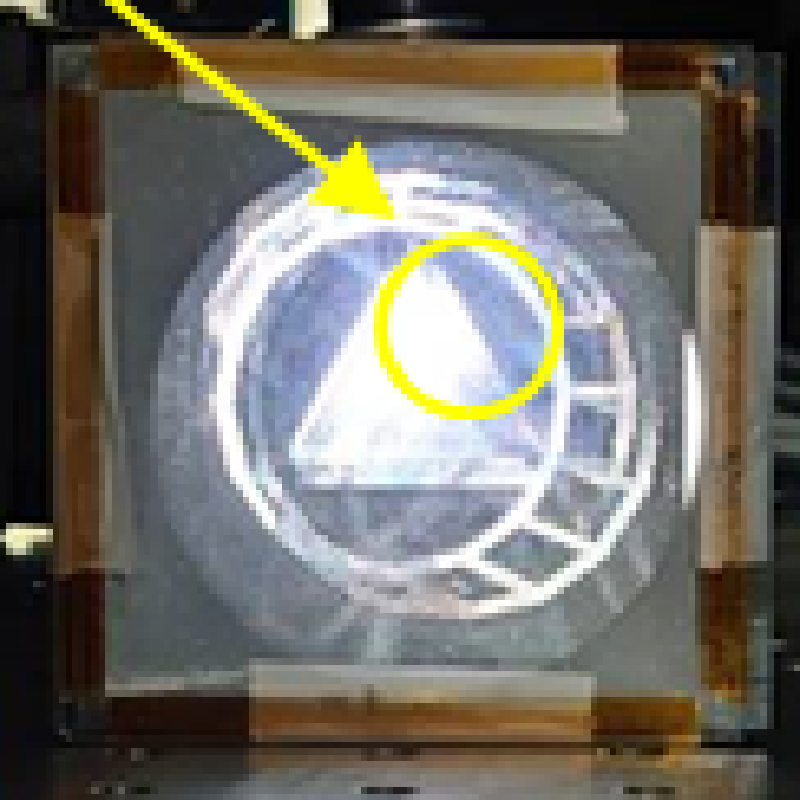
\includegraphics[width=0.3\textwidth]{img/imperfections-3.png}
                }
                \caption{Imperfection examples}
            }
            \setcounter{figure}{4}
            \only<4>{
                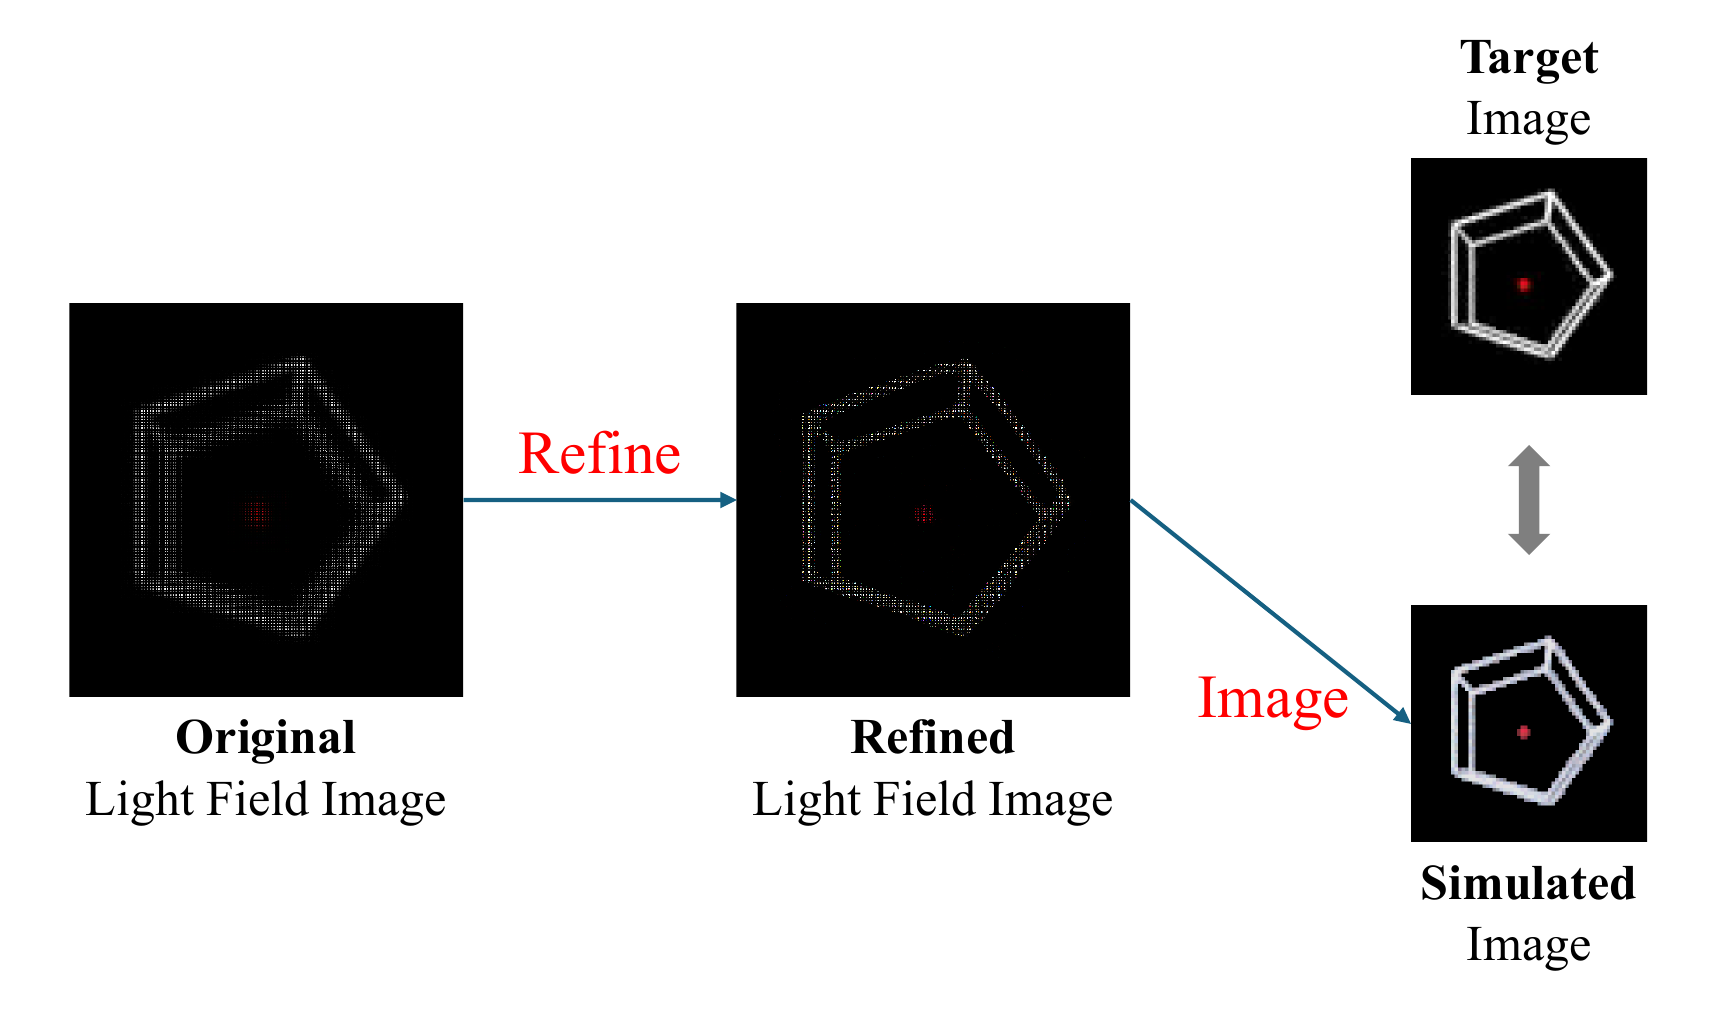
\includegraphics[width=0.8\textwidth]{img/_method-1.png}
                \caption{Overview of our two-stage method}
            }
            \setcounter{figure}{5}
            \only<5>{
                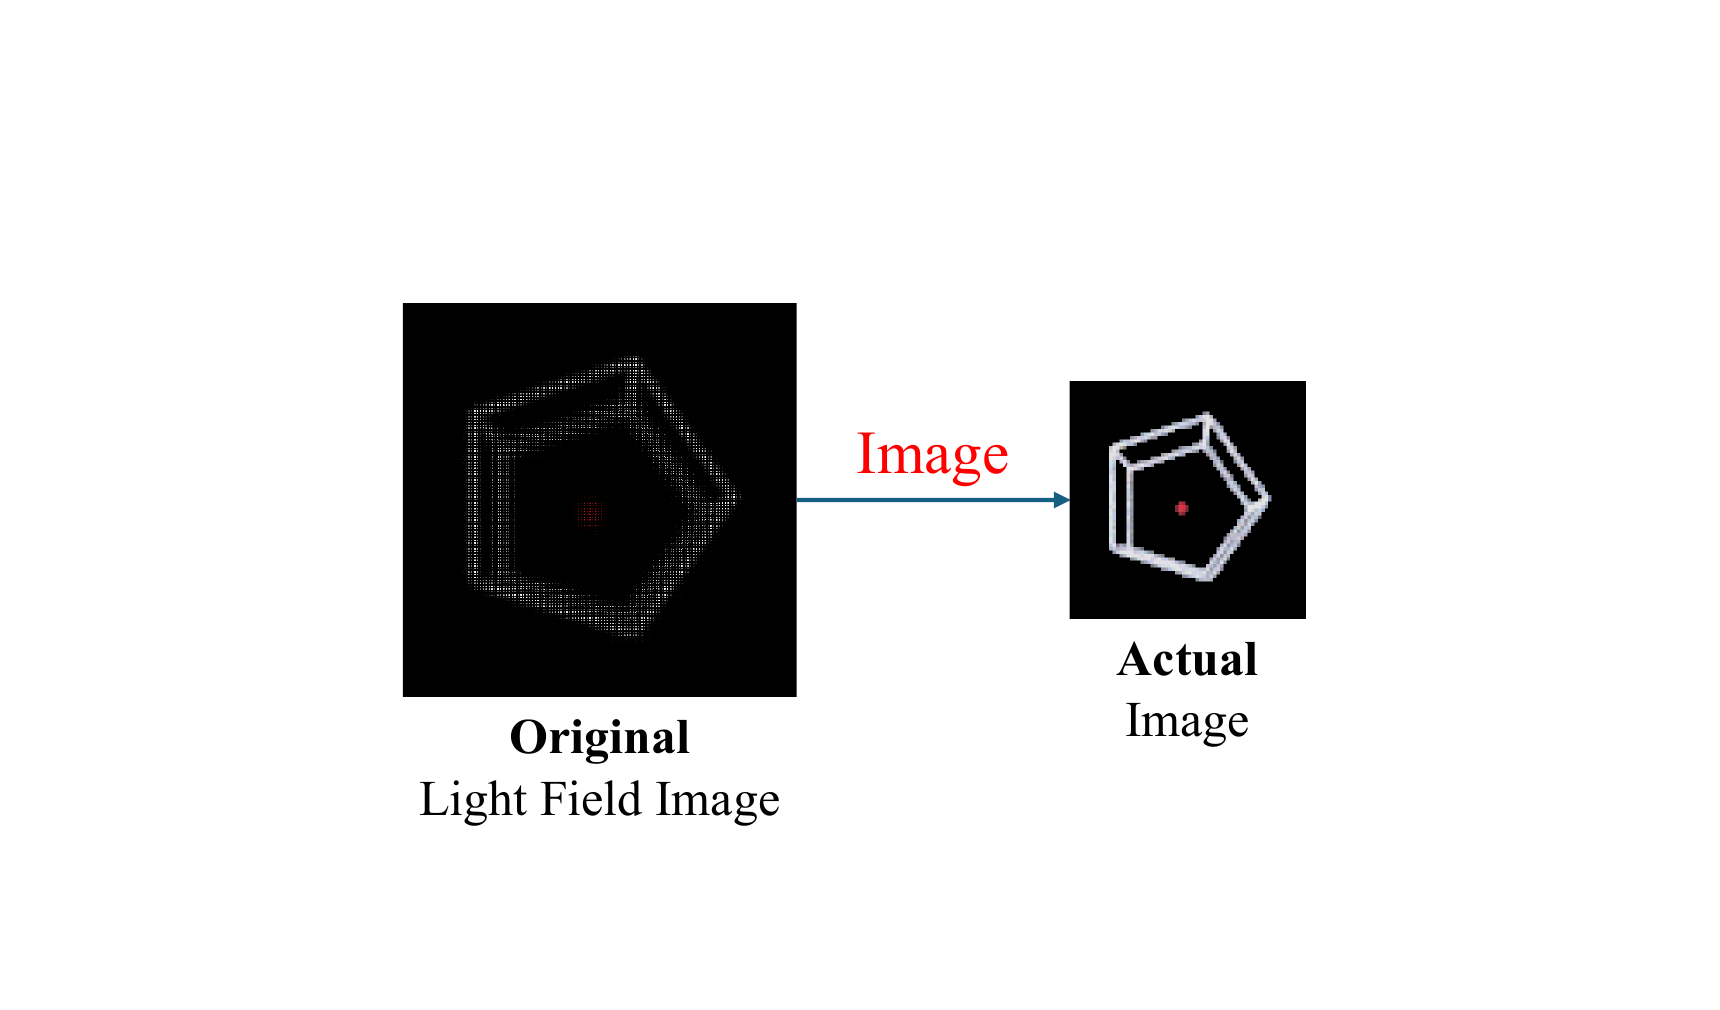
\includegraphics[width=0.8\textwidth]{img/_method-2.png}
                \caption{First-stage of our method}
            }
            \setcounter{figure}{6}
            \only<6>{
                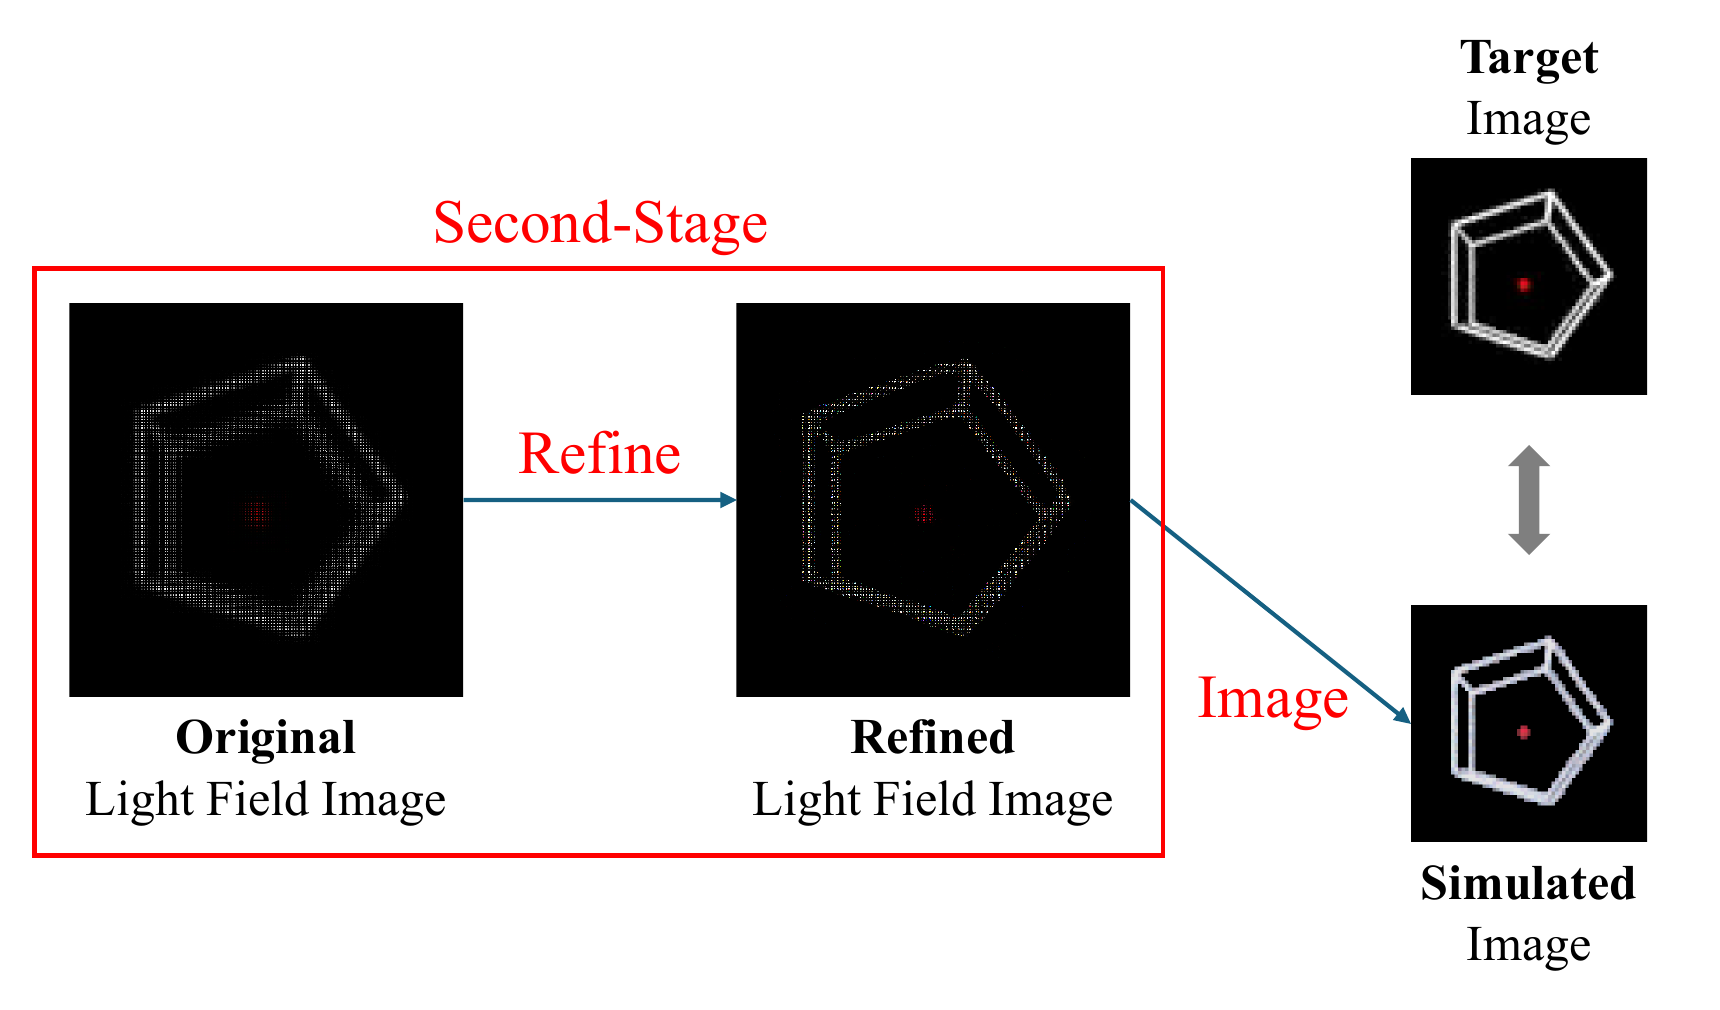
\includegraphics[width=0.8\textwidth]{img/_method-3.png}
                \caption{Second-stage of our method}
            }
            \setcounter{figure}{7}
            \only<7>{
                \subfigure[Target image]{
                    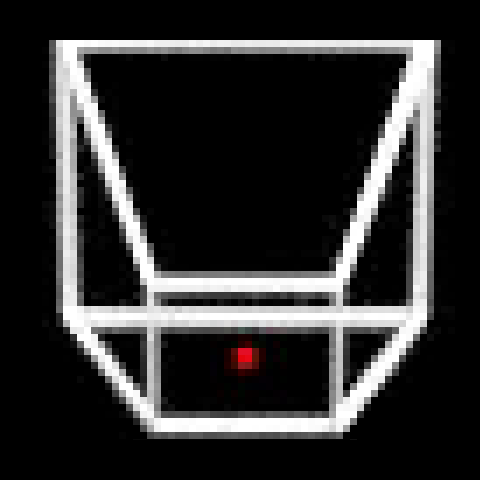
\includegraphics[width=0.3\textwidth]{img/00091_view3_vpi_img.png}
                }
                \subfigure[Original actual image]{
                    
\includegraphics[width=0.3\textwidth]{img/00091_view3_calX_img_real.png}
                }
                \subfigure[\ctextbf{Simulated} image after refinement]{
                    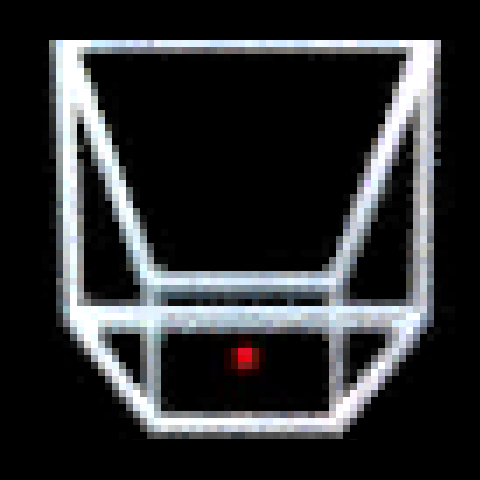
\includegraphics[width=0.3\textwidth]{img/00091_view3_calY_img_sim_k21.png}
                }
                \caption{Light field image refinement sample 1}
            }
            \only<8>{
                \subfigure[Target image]{
                    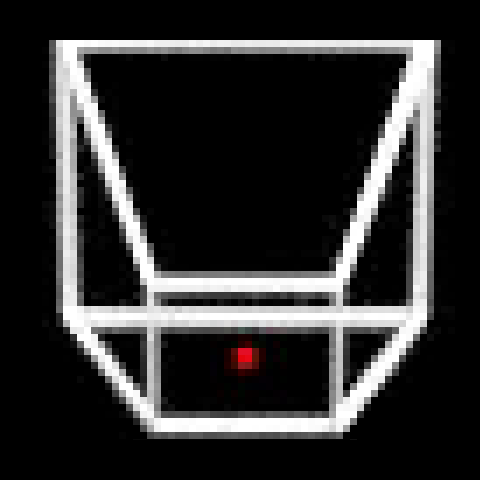
\includegraphics[width=0.3\textwidth]{img/00091_view3_vpi_img.png}
                }
                \subfigure[Original actual image]{
                    
\includegraphics[width=0.3\textwidth]{img/00091_view3_calX_img_real.png}
                }
                \subfigure[\ctextbf{Actual} image after refinement]{
                    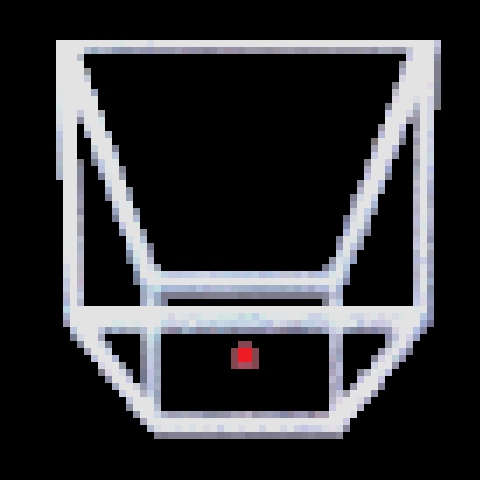
\includegraphics[width=0.3\textwidth]{img/00091_view3_calY_img_real_k21.png}
                }
                \caption{Light field image refinement sample 1}
            }
            \only<9>{
                \subfigure[Target image]{
                    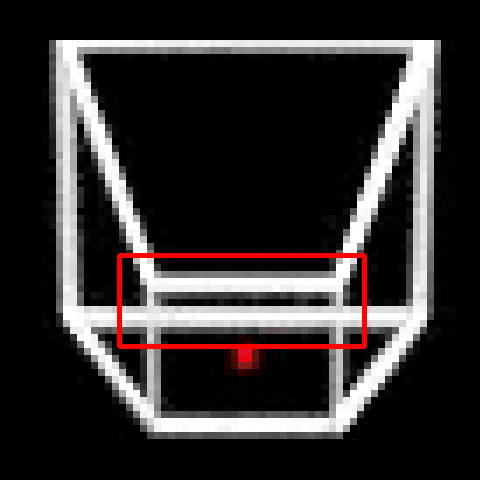
\includegraphics[width=0.3\textwidth]{img/00091_view3_vpi_img_box.png}
                }
                \subfigure[Original actual image]{
                    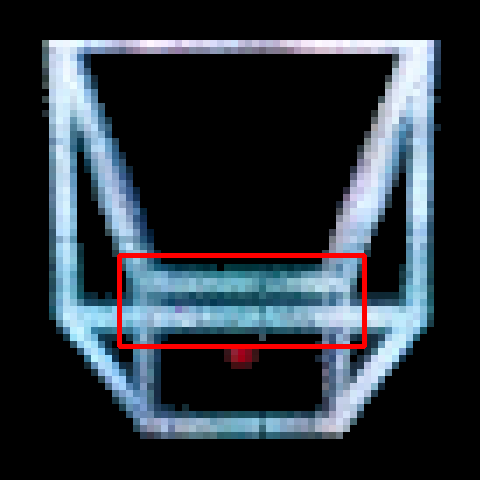
\includegraphics[width=0.3\textwidth]{img/00091_view3_calX_img_real_box.png}
                }
                \subfigure[\ctextbf{Actual} image after refinement]{
                    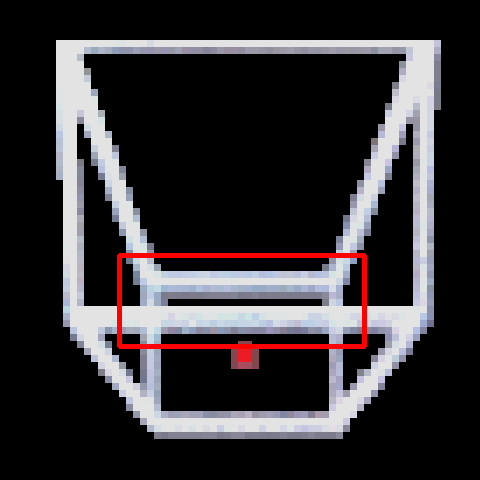
\includegraphics[width=0.3\textwidth]{img/00091_view3_calY_img_real_k21_box.png}
                }
                \caption{Light field image refinement sample 1}
            }

            \setcounter{figure}{8}
            \only<10>{
                \subfigure[Target image]{
                    
\includegraphics[width=0.3\textwidth]{img/00460_view4_vpi_img.png}
                }
                \subfigure[Original actual image]{
                    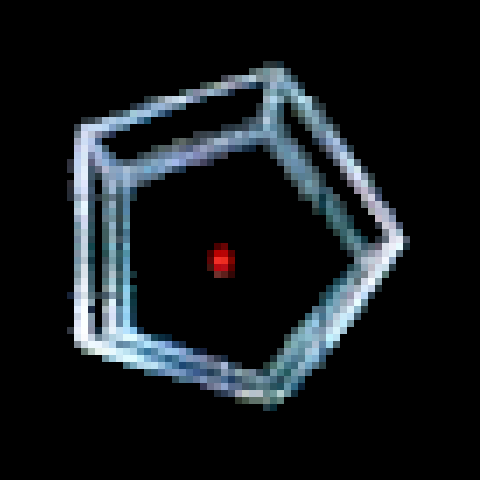
\includegraphics[width=0.3\textwidth]{img/00460_view4_calX_img_real.png}
                }
                \subfigure[\ctextbf{Simulated} image after refinement]{
                    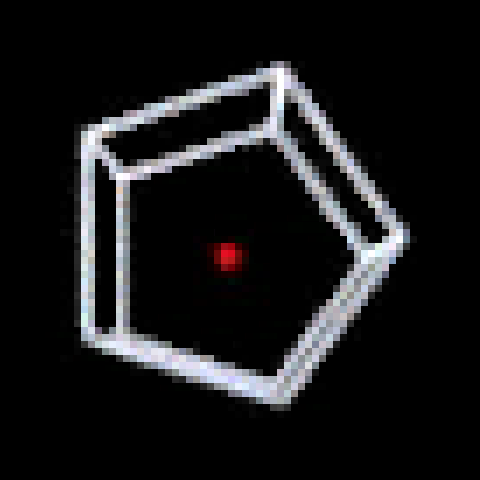
\includegraphics[width=0.3\textwidth]{img/00460_view4_calY_img_sim_k21.png}
                }
                \caption{Light field image refinement sample 2}
            }
            \only<11>{
                \subfigure[Target image]{
                    
\includegraphics[width=0.3\textwidth]{img/00460_view4_vpi_img.png}
                }
                \subfigure[Original actual image]{
                    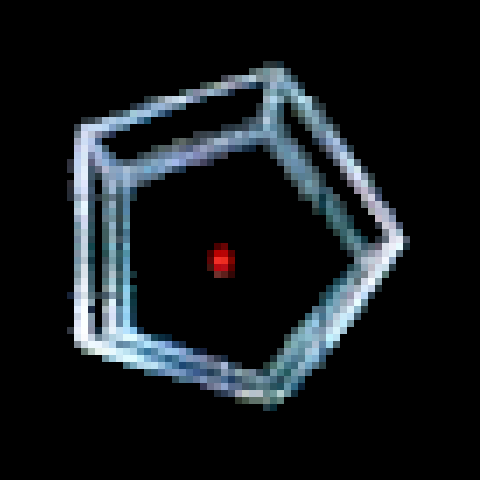
\includegraphics[width=0.3\textwidth]{img/00460_view4_calX_img_real.png}
                }
                \subfigure[\ctextbf{Actual} image after refinement]{
                    
\includegraphics[width=0.3\textwidth]{img/00460_view4_calY_img_real_k21.png}
                }
                \caption{Light field image refinement sample 2}
            }
            \only<12>{
                \subfigure[Target image]{
                    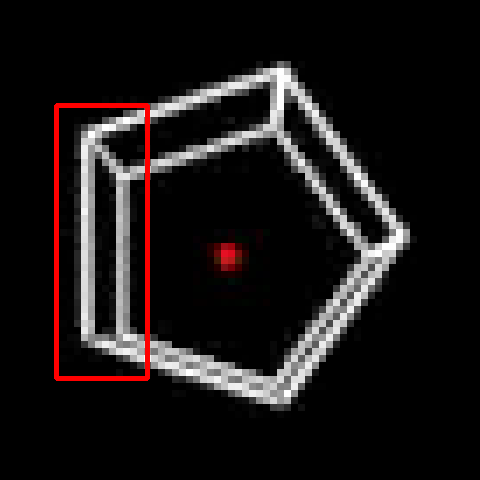
\includegraphics[width=0.3\textwidth]{img/00460_view4_vpi_img_box.png}
                }
                \subfigure[Original actual image]{
                    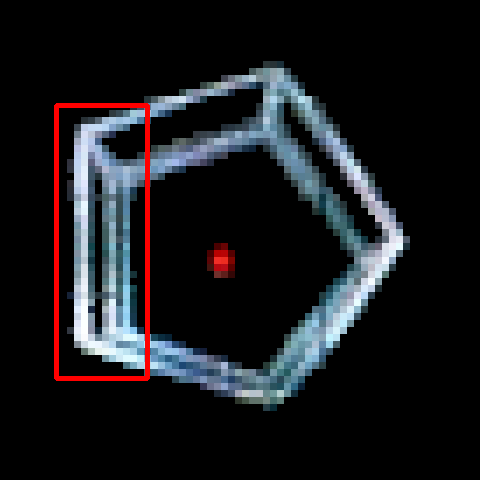
\includegraphics[width=0.3\textwidth]{img/00460_view4_calX_img_real_box.png}
                }
                \subfigure[\ctextbf{Actual} image after refinement]{
                    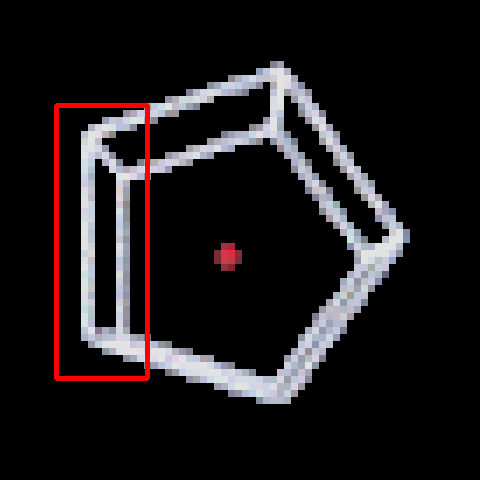
\includegraphics[width=0.3\textwidth]{img/00460_view4_calY_img_real_k21_box.png}
                }
                \caption{Light field image refinement sample 2}
            }
        \end{figure}
    \end{block}
\end{frame}

%----------------------------------------------------------------------------------------
%	AWARDS SLIDES
%----------------------------------------------------------------------------------------

% \section{Awards}
% \begin{frame}
%     \frametitle{Awards}
%     \begin{block}{CCCC-Mobile Application Innovation Contest}
%         First Prize \hfill 09 2018
%     \end{block}
%     \begin{block}{The 4th ”Internet+” Innovation and Entrepreneurship Competition}
%         Gold Award \hfill 09 2018
%     \end{block}
%     \begin{block}{College Students’ Innovative Entrepreneurial Training Plan Program (SRTP)}
%         Excellent \hfill 04 2018 – 05 2019
%     \end{block}
% \end{frame}

%----------------------------------------------------------------------------------------
%	EXPERIENCE SLIDES
%----------------------------------------------------------------------------------------

% \section{Experience}
% \begin{frame}
%     \frametitle{Experience}
%     \begin{block}{The University of British Columbia Vancouver Summer Program}
%         Vancouver, Canada \hfill 07 2019 – 08 2019
%         \begin{itemize}
%             \item Included 2 courses, ”Algorithms and the World Wide Web” and ”Building Modern Web Applications”.
%             \item Collaborated with my teammates to complete our projects as team leader.
%         \end{itemize}
%     \end{block}
% \end{frame}

%----------------------------------------------------------------------------------------
%	SKILLS SLIDES
%----------------------------------------------------------------------------------------

% \section{Skills}
% \begin{frame}
%     \frametitle{Skills}
%     \begin{block}{Languages}
%         Python, Java, C, JavaScript
%     \end{block}
%     \begin{block}{Technologies/Frameworks}
%         PyTorch, Flask, Spring Boot, Vue.js, Git, SQL, MongoDB
%     \end{block}
% \end{frame}

\section{Thanks}
\begin{frame}
    \begin{center}
        \huge{\texttt{Thanks for your attention}} \\~\\
        \LARGE{許子駿} \\ \Large{Oscar} \\
        \vspace{16pt}
        \scriptsize{
            \href{tel:+886-987605719}{ \raisebox{-0.1\height}\faPhone\ \underline{+886-987605719} ~} 
            \href{mailto:vm3y3rmp40719@gmail.com}{\raisebox{-0.2\height}\faEnvelope\  \underline{tzuchunhsu@realtek.com}} \\~\\
            \href{https://www.linkedin.com/in/tzu-chun-hsu-ab4b3b188/}{\raisebox{-0.2\height}\faLinkedinSquare\ \underline{tzu-chun-hsu-ab4b3b188} ~}
            \href{https://github.com/Oscarshu0719}{\raisebox{-0.2\height}\faGithub\ \underline{Oscarshu0719}}
        }
    \end{center}
\end{frame}
\end{document}